\chapter{Chemistry on a Computer}
\newcommand{\schro}{Schr\"{o}dinger}
\label{chapter:theory}
\section{Quantum Mechanics and Chemistry}\label{section: theory}
\subsection{Overview}\label{section: theory_overview}
The development of quantum mechanics in the early 20th century armed scientists with the tools to calculate the microscopic properties of matter. In chemistry, the postulates of quantum mechanics can be applied to calculate relative energies of molecules, molecular geometries, ratios of products of chemical reactions, transition states, spectra, and any other phenomenon of interest. However, whilst in principle any property can be calculated exactly by the \schro{} equation, the analytical solution is only obtainable for systems with one electron. For systems larger than this, and therefore anything of observable chemical relevance, the computational expense on even modern computer architecture is intractable. 

To overcome this, a number of approximations are used field of computational chemistry. In general, as the number of atoms one wants to model increases, qualitative nature of the result also increases. Computational chemistry methods can generally be split into the types of approximations made and the number of atoms the method wishes to treat. In biophysical process and the modelling of proteins on the scale of tens of thousands of atoms, quantum mechanics (and electrons) are ignored completely. Forcefields are used to calculate the energy corresponding to a set of atomic coordinates in what are known as the \ac{MM} class of methods. The interactions between atoms are defined by analytical potentials, such as for bond stretches, bends, and angles, and are parameterised for different types of molecules using more accurate methods. This procedure is time-consuming and makes the forcefield specific to the systems it was fitted to, but enables computationally facile access to molecular geometries and properties of large systems.

At the other end of the scale, for systems of typically less than 500-1000 atoms, the electronic structure is included through wavefunction and \ac{DFT} techniques. For the applications involved in this thesis, involving photoinduced phenomena, the activity of the electrons is paramount, and as such it is these methods which are utilised herein. In the next sections, the importance of the \schro{} equation shall be established, which along with the Born-Oppenheimer approximation enables the calculation of electronic properties through the simplest wavefunction method, the \ac{HF} method. 
%%%%%%%%%%%%%%
%%%%%%%%%%%%%%
\subsection{The \schro{} Equation}\label{section: theory_schrodinger}
%%%%%%%%%%%%%%
%%%%%%%%%%%%%%
The wavefunction $\Psi$ contains all the information about the quantum state of the system at a position and time. As Newton's second law ($\bm{\mathrm{F}}=m\bm{\mathrm{a}}$) gives a classical particle's position and moment at each time period, thus describing it's classical state, so the time-dependent \schro{} equation does for wavefunction, and has the general form
\begin{equation}\label{equation: td-schro}
    i\hbar{}\frac{\partial \Psi(r,t)}{\partial t}=\hat{H}\Psi(r,t)
\end{equation}
where $\hbar=\frac{h}{2\pi}$ and $\hat{H}$ is the Hamiltonian operator. Separating the spatial ($r$) part from the temporal ($t$) part of differential time-dependent \schro{} equation yields the time-dependent version of the \schro{} equation, which using the bra-ket notation of Dirac is
\begin{equation}\label{equation: ti-schro}
   \hat{H}\ket{\Psi}=E\ket{\Psi}.
\end{equation}
This is an eigenvalue equation, where the Hamiltonian operator acts on the wavefunction to give the energy $E$ of the system. For a system of $N$ electrons described by position vectors $\bm{r}$ and $M$ nuclei with position vectors $\bm{R}$, the Hamiltonian calculates the kinetic ($T$) and potential ($V$) energy contributions of the electrons and nuclie towards the total energy of the system
\begin{equation}\label{equation: H-simple}
\hat{H}=\hat{T}_{e}+\hat{T}_{n}+\hat{V}_{n-e}+\hat{V}_{e-e}+\hat{V}_{n-n}
\end{equation}
\begin{equation}\label{equation: H}
   \hat{H}=\underbrace{-\sum_{i=1}^{N}\frac{1}{2}\nabla_{i}^2 - \sum_{A=1}^{M}\frac{1}{2M_{A}}\nabla_{A}^2}_\text{kinetic terms}-\underbrace{\sum_{i=1}^{N}\sum_{A=1}^{M}\frac{Z_{A}}{r_{iA}}+\sum_{i=1}^{N}\sum_{j>{i}}^{N}\frac{1}{r_{ij}}+\sum_{A=1}^{M}\sum_{B>{A}}^{M}\frac{Z_{A}Z_{B}}{R_{AB}}}_\text{electrostatic terms}.
\end{equation}
$i$ and $j$ are electrons and $A$ and $B$ are nuclei. The first two terms are the operators for the kinetic energy of the electrons and the nuclei, where the Laplacian operator $\nabla^{2}$ is the second derivative of position. The next three terms are the electrostatic operators, summing the Coulomb interactions in the system;  the attractive interaction between electrons and the nuclei (of charge $Z$); the repulsive interaction between electrons; and the repulsive interaction between nuclei. Atomic units are used throughout, such that the electronic charge and mass are neglected. The $R$ and $r$ terms in the electrostatic parts denote the distance between nuclei and electrons.  To calculate the energy $E$ , however, an eigenfunction for Equation \ref{equation: ti-schro}
is required, corresponding to a wavefunction describing the electronic state.\cite{aszabo82:qchem}

In the hydrogen atom, the $\hat{V}_{e-e}$ and $\hat{V}_{n-n}$ can be neglected since there is only one proton and one electron, and the exact solution for the energy can be calculated since the wavefunction can be constructed analytically. However, for larger systems with many electrons and nuclei, Equation \ref{equation: ti-schro} cannot be solved. As such, a number of approximations must be made. The most fundamental of these is Born-Oppenheimer approximation, which shall be introduced in the next section.
%%%%%%%%%%%%%%
%%%%%%%%%%%%%%
\subsection{The Born-Oppenheimer Approximation}\label{section: theory_bornoppenheimer}
%%%%%%%%%%%%%%
%%%%%%%%%%%%%%
Separation of variables is a key concept in quantum chemistry, where a complex problem is broken down into constituent parts. This method is used to simply the solving of Equation \ref{equation: ti-schro} by separating the electronic terms from the nuclear terms. This is rooted in the fact that the nuclei are vastly heavier than electrons, and so it can be approximated that the nuclei are static with respect to the electrons. Equation \ref{equation: ti-schro} is solved, then, in two steps. First, the electronic structure is solved with ``clamped" nuclei, resulting in an electronic energy which is a parametric function of the nuclear coordinates. By concentrating on just the electronic terms, the \textit{electronic} Hamiltonian $\hat{H}_{e}$ becomes
\begin{equation}\label{equation: Hel}
     \hat{H}_{e}=\underbrace{-\sum_{i=1}^{N}\frac{1}{2}\nabla_{i}^2}_\text{kinetic term}-\underbrace{\sum_{i=1}^{N}\sum_{A=1}^{M}\frac{Z_{A}}{r_{iA}}+\sum_{i=1}^{N}\sum_{j>{i}}^{N}\frac{1}{r_{ij}}}_\text{electrostatic terms}.
\end{equation}
and the electronic \schro{} equation is then
\begin{equation}\label{equation: ti-schro-el}
   \hat{H}_{e}\ket{\Phi}=E_{e}\ket{\Phi}
\end{equation}
where $\Phi$ is the electronic wavefunction. In similar fashion, the nuclear wavefunction is solved for the nuclei in the average field of the electrons. The nuclear motion is thus determined by the electronic energy, and the nuclei move on a \ac{PES}. The total wavefunction is a product of the electronic and nuclear wavefunctions. Whilst the Born-Oppenheimer approximation helps divide the problem, solving the electronic problem exactly for many electron systems is impossible. The \acf{HF} method is the fundamental quantum chemical approach to solve the many electron problem.
%%%%%%%%%%%%%%
%%%%%%%%%%%%%%
\subsection{The Hartee-Fock Method}\label{section: theory_HF}
%%%%%%%%%%%%%%
%%%%%%%%%%%%%%
In the \ac{HF} method, the intractable $N$-electron wavefunction $\Phi$ is simplified to be a product of $N$, one-electron wavefunctions $\chi$,
\begin{equation}
\ket{\Phi}=\ket{\chi_{1}\chi_{2}...\chi_{i}..\chi_{N}}.
\end{equation}
 where $\chi$ are spin orbitals of each electron in the system. The spin orbitals consist of a spatial functional and a spin function, an infinite number of which will provide an exact solution. However, in practical terms a basis set is supplied, where molecular orbitals are made of (typically) linear combination of Gaussian functions, representing atomic orbitals. Whilst Gaussian functions themselves do not reflect the correct atomic orbital behaviour seen in Slater-type functions, the combination of multiple Gaussians can recover the radial behaviour along with the many numerical advantages. 
 
 From the Pauli exclusion principle, no two electrons may share exactly the same four quantum numbers (i.e occupy the same spatial and spin orbital). Since electrons are fermions, the electronic wavefunction is \textit{antisymmetric}, meaning that a change in the orbital must result in the wavefunction changing sign. This is enforced using Slater Determinants. This is most easily seen for a two-electron system for electrons at positions $\bm{x}_{1}$ and $\bm{x}_{2}$, where orbital $\chi_{1}$ contains electron at $\bm{x}_1$ and orbital $\chi_{2}$ contains electron at $\bm{x}_2$, with a normalisation factor of $N^{-\frac{1}{2}}$
\begin{equation}
\begin{split}
\Phi(\bm{x}_{1},\bm{x}_{2})&=\frac{1}{\sqrt{2}}\{\chi_{1}(\bm{x}_{1})\chi_{2}(\bm{x}_{2})-\chi_{1}(\bm{x}_{2})\chi_{2}(\bm{x}_{1})\}\\
&=\frac{1}{\sqrt{2}}
\begin{vmatrix}
\chi_{1}(\bm{x}_{1})&\chi_{2}(\bm{x}_{1})\\
\chi_{1}(\bm{x}_{2})&\chi_{2}(\bm{x}_{2})
\end{vmatrix}
\end{split}
\end{equation}
where by taking the determinant, the antisymmetry is ensured since putting the electron exchanging the electrons changes the sign of the determinant. In the determinant, the rows consist of the electrons while the columns contain the orbitals. In the \ac{HF} method, the wavefunction is approximated by a single Slater Determinant, and therefore \ac{HF} is known as a single-determinant, or single-reference, method.  As well as ensuring antisymmetry, the Slater determinant wavefunction also introduces exchange correlation, where the motion of two electrons with the same spin is correlated. This means that the probability of finding one electron at a certain position is dependent on the position of an electron of the same spin at another position, and the probability of finding the two electrons at the \textit{same} point in space in zero. This is not true for electrons of opposing spin, and thus antiparallel spins are uncorrelated in the \ac{HF} method.

The electronic energy of the wavefunction is an expectation value of $\hat{H}_{e}$, such that
\begin{equation}\label{equation: energy_expectation}
E=\bra{\Phi}\hat{H_e}\ket{\Phi}.
\end{equation}
The variational principle states that the true ground state wavefunction will always be less than or equal to a trial wavefunction, meaning that the guessed spin orbitals will never undershoot the true energy. As such, 
\ac{HF} is a purely iterative method where the energy is computed for a set of trial spin orbitals, the spin orbitals are altered, and the energy is guessed again. This is repeated until convergence. 

To calculate the ``best" set of orbitals, the interactions in the electronic Hamiltonian are split into one-electron and two electron terms. The one electron terms are collected by the core Hamiltonian operator $\hat{h}_{i}$, involving the kinetic energy of the electrons and the electron-nuclei interactions,
\begin{equation}
    \hat{h}_{i}=-\frac{1}{2}\nabla_{i}^{2}-\sum_{A=1}^{M}\frac{Z_{A}}{r_{iA}}.
\end{equation}
The antisymmetric nature of the Slater determinent results in two operators for the electron-electron interaction, a Coulomb operator $\hat{J}_{ij}$ and an exchange operator $K_{ij}$, which act on orbital $\chi_{i}$ to determine the effect of the remaining orbitals,
\begin{equation}
    \hat{J}_{ij}\chi_{i}=\chi_{i}\int{\frac{\chi^{\ast}_{j}\chi_{j}}{r_{ij}}d\bm{x}_{2}}
\end{equation}
\begin{equation}
    \hat{K}_{ij}\chi_{i}=\chi_{j}\int{\frac{\chi^{\ast}_{j}\chi_{i}}{r_{ij}}d\bm{x}_{2}}.
\end{equation}
The Coulomb operator determines the Coulomb potential felt by electron $i$ in orbital $\chi_{i}$ from electron $j$ in orbital $\chi_{j}$. This is done by \textit{averaging} the interaction over all of the spatial coordinates of electron $j$. As such, $J_{ij}$ represents the average, or \textit{mean-field}, local potential felt by electron $i$. For this reason, the \ac{HF} method is often called a mean-field approach. The exchange operator $K_{ij}$ is a result of the antisymmetric Slater determinant, and is a quantum mechanical artefact of the fact that electrons are by nature  indistinguishable, and the exact labelling ($i$,$j$) has no physical meaning. 

The one-electron and two-electron operators are collected by the Fock operator $\hat{F}$, such that
\begin{equation}
    \hat{F}=\hat{h_{i}}+\sum_{j\neq{}i}^{\frac{N}{2}}{[\hat{J_{ij}}-\hat{K_{ij}}]}
\end{equation}
The two electron terms run over only half of the electrons ($\frac{N}{2}$ to ensure interactions are not double counted, while the condition of $j\neq{}i$ means that an electron cannot interact with itself. 

The Fock operator allows Equation \ref{equation: ti-schro} to be solved in the \ac{HF} method through,
\begin{equation}\label{equation: Fock-operator}
    \hat{F}\ket{\Phi}=E\ket{\Phi}
\end{equation}
an eigenvalue equation solved by altering the linear combination of basis functions until energy convergence is reached. In practice, for a closed shell system, the molecular orbital $\chi_{i}$ consists of a linear combination of $K$ atomic basis functions,
\begin{equation}\label{equation: expansion}
    \chi_{i}=\sum_{\mu=1}^{K}C_{ui}\phi_{\mu}\qquad\quad{}i=1,2,..,K
\end{equation}
The Roothaan equations are then used to solve Equation \ref{equation: Fock-operator} in matrix form,
\begin{equation}
    \bm{FC}={\bm{SC\epsilon}}
\end{equation}
where $\bm{F}$ is the Fock matrix containing the elements from the Fock operator, $\bm{C}$ contains the expansion coefficients from Equation \ref{equation: expansion} and $\bm{S}$ is the overlap matrix containing the overlaps of atomic orbitals ($\bra{\phi_{i}}\ket{\phi_{j}}$). By diagonalising the Fock matrix, $\epsilon$ is a diagonal matrix containing the orbital energies. \ac{HF} is commonly named the self-consistent field approximation, since the Roothaan equations are solved until self-consistency is reached.


The \ac{HF} method is a powerful approach to solving the electronic part of the \schro{} equation. However, it has several severe drawbacks which hinder its application and have resulted in more sophisticated methods being developed to address the shortcomings within. The most serious of these for ground state, closed-shell systems is the correlation problem. While electrons of parallel spin have the required exchange correlation, the Coulomb correlation is completely neglected since each electron sees only an average field of the other electrons. In reality, the motion of one electron is dependent on the motion of each of the other electrons (Figure \ref{figure: mean-field}), and the energy of the system in \ac{HF} is overestimated in respect to the true energy. A number of methods to overcome the lack of correlation have been developed, which use the \ac{HF} method as a starting point before calculating the electron correlation. These are called post-Hartree-Fock methods, and those most relevant to the work in this thesis are discussed in the next section.
\begin{figure}[H]
\centering
  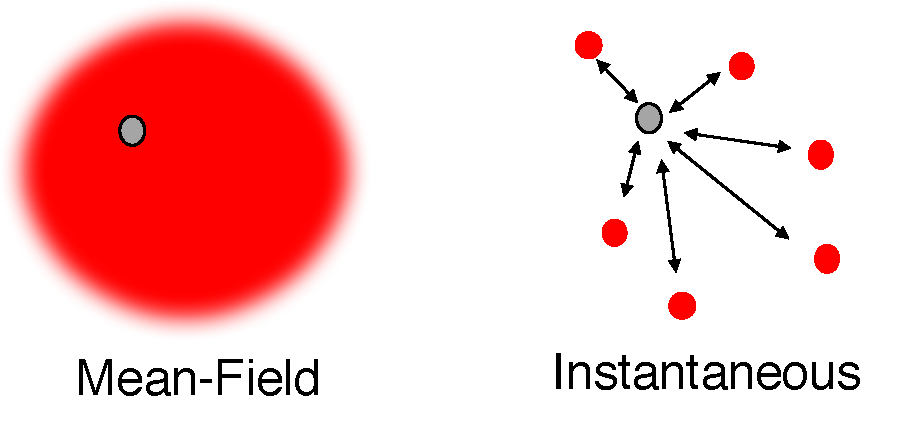
\includegraphics[width=0.4\linewidth]{Theory/Mean_Field.pdf}
  \caption[Schematic of the mean-field approximation]{Depiction of the mean field electron interaction, where the electron of interest interactions with an average potential, rather than individually with each other electron.}
  \label{figure: mean-field}
\end{figure}
%%%%%%%%%%%%%%
%%%%%%%%%%%%%%
\subsection{Post-Hartre-Fock Methods}\label{section: theory_postHF}
%%%%%%%%%%%%%%
%%%%%%%%%%%%%%
\subsubsection{M{\o}ller-Plesset Perturbation Theory}
%%%%%%%%%%%%%%
Electron correlation energy can be added to the \ac{HF} energy by way of an external perturbative correction. In perturbation theory, the total Hamiltonian is divided into the zeoth-order part $\hat{H}_{0}$, which is the \ac{HF} Hamiltonian, and a perturbation $\hat{V}$, such that the eigenvalue equation becomes
\begin{equation}\label{equation: PT}
    \hat{H}\ket{\Phi_{i}}=(\hat{H}_{0}+\hat{V})\ket{\Phi_{i}}=\epsilon_{i}\ket{\Phi_{i}}.
\end{equation}
The eigenvalues and eigenfunctions of $\hat{H}_{0}$ so that they become closer to the total Hamiltonian $\hat{H}$, which would then contain electronic correlation. This is done by the ordering factor $\lambda$, such that
\begin{equation}
    \hat{H}=\hat{H}_{0}+\lambda\hat{V}
\end{equation}
The true eigenvalues and eigenfunctions are expanded in a Taylor series in $\lambda$ up to $n$th order,
\begin{equation}\label{equation: MP2_energies}
    \epsilon_{i}=E_{i}^{(0)}+\lambda{}E_{i}^{(1)}+\lambda^{2}E_{i}^{(2)}+\lambda^{3}E_{i}^{(3)}+..+\lambda^{n}E_{i}^{(n)}
\end{equation}
\begin{equation}\label{equation: MP2_functions}
    \ket{\Phi_{i}}=\ket{\Phi_{i}^{(0)}}+\lambda{}\ket{\Phi_{i}^{(1)}}+\lambda^{2}\ket{\Phi_{i}^{(2)}}+\lambda^{3}\ket{\Phi_{i}^{(3)}}+..+\lambda^{n}\ket{\Phi_{i}^{(n)}}
\end{equation}
After inserting Equations \ref{equation: MP2_energies} and \ref{equation: MP2_functions} into Equation \ref{equation: PT} and collecting terms by order, the general expression for the total energy is
\begin{equation}
E_{i}=E_{i}^{(0)}+\sum_{n=1}^{n}\bra{\Phi_{i}^{(0)}}\hat{V}\ket{\Phi_{i}^{(n-1)}}
\end{equation}
The perturbation operator $\hat{V}$ introduces the Coulomb repulsion between electrons, which when combined with excited Slater determinants, recovers the correlation energy. In most chemical applications, the method is contracted at second-order, and was initially employed by C. M{\o}ller and M.S. Plesset to obtain the correlation energy, hence the acronym \ac{MP2} is often used.\cite{Moller1934} Since MP is perturbative, the MP-calculated energy can be lower than the true energy, making it a non-variational method.
%%%%%%%%%%%%%%
\subsubsection{Coupled Cluster Theories}
%%%%%%%%%%%%%%
In an alternative approach to perturbation theory, \ac{CC} methods were introduced in the 1960s to account for electron correlation.\cite{Cizek1966,Paldus1972} \ac{CC} theory uses excited determinants by means of a Taylor expansion with an exponential operator
\begin{equation}\label{equation: cc}
    \ket{\Phi_{CC}}=e^{\hat{T}}\ket{\Phi_{0}}
\end{equation}
where $\ket{\Phi_{0}}$ is the \ac{HF} wavefunction nad $\hat{T}$ is the cluster operator. The cluster operator produces a sum of excitation operators up to the truncation level $n$
\begin{equation}\label{equation: T}
    \hat{T}=\hat{T}^{(1)}+\hat{T}^{(2)}\hat{T}^{(3)}+..+\hat{T}^{(n)}
\end{equation}
where $N$ is the excitation number. So, $\hat{T}^{(1)}$, includes all single excitations and $\hat{T}^{(1)}$ includes all double excitations, \textit{etc}. For the first order, the contribution of all single excited determinants is 
\begin{equation}
    \hat{T}^{(1)}\ket{\Phi_{0}}=\sum_{i}^{occ}\sum_{a}^{vir}t_{i}^{a}\phi_{i}^{a}
\end{equation}
where $\phi_{i}^{a}$ is the excitation of an electron from occupied orbital $\phi_{i}$ to virtual orbital $\phi_{a}$, and $t_{i}^{a}$ is the amplitude given to this exctitation. Substituting \ref{equation: T} into \ref{equation: cc} yields the coupled cluster wavefunction
\begin{equation}\label{equation: CCwavefunctioncomplete}
\ket{\Phi_{CC}}=e^{\hat{T}}\ket{\Phi_{0}}=\big[1+\hat{T}^{(1)}+(\hat{T}^{(2)}+\frac{\hat{T}^{2(1)}}{2})+(\hat{T}^{(3)}+\hat{T}^{(2)}\hat{T}^{(1)}+\frac{\hat{T}^{3(1)}}{6})\big]\Phi_{0}
\end{equation}
As for perturbation theory, \ac{CC} theory is usually referred to by the trunctation level, for example CCSD refers to coupled cluster with single and double excitations. CCSD scales at $N^{6}$, adding considerable expense to the \ac{HF} method, which scales at $N^{4}$.

In this thesis, approximate \ac{CC} methods are used to calculate excited state properties of molecules, namely the \ac{CC}2 method. The \ac{CC}2 method was formulated in 1995 to approximate CCSD but with $N^{5}$ scaling and provide accurate excitation energies.\cite{Christiansen1995} In \ac{CC}2, the single excitations of CCSD are retained by the double excitations are approximated, with comparable ground state accuracy of MP2. Response functions of \ac{CC}2 provide excitation energies and transition moments, making it a popular method in probing excited-state properties of molecules.\cite{Sneskov2012}

As an alternative but closely related approach, propagator methods are also used to calculate excitation energies and transtion moments. The polarizer propagator introduces the effect of an external field, for instance the absorption of a photon. In the \ac{ADC2}, the polarizer propagator acts on the \ac{MP2} ground state to give excitation energies at similar accuracy but reduced computational cost compared to \ac{CC}2.
%%%%%%%%%%%%%%
\subsection{Multiconfigurational Methods}\label{section: theory_multiconf}
%%%%%%%%%%%%%%